\documentclass[conference,compsoc]{IEEEtran}

\usepackage{cite}
\usepackage{booktabs}
\usepackage{multirow}
\usepackage{graphicx}
\usepackage{siunitx}
\usepackage{amsmath}
\usepackage{amssymb}
\usepackage{enumitem}
\usepackage{hyperref}
\usepackage{microtype}
\newcommand{\Description}[1]{}

\title{Calibrated and Auditable Window-Level Network Intrusion Detection with TCN-WGAN-GP}

\author{\IEEEauthorblockN{Anonymous Submission}}

\begin{document}
\maketitle

\begin{abstract}
Network Intrusion Detection Systems (NIDS) are ultimately consumed as alarm streams, where excessive benign alerts increase analyst workload and alert fatigue. This paper studies window-level intrusion detection as a calibrated alarm-generation problem rather than only as offline score ranking. We present a pipeline based on a Temporal Convolutional Network Wasserstein Generative Adversarial Network with Gradient Penalty (TCN-WGAN-GP) and fused Temporal Attention-Deviation (TAD) scoring.

The method couples anomaly scoring with a strict no-leakage calibration design: scaler fitting, benign-only model training, benign-reference construction, threshold calibration, and final testing are assigned separate data roles. The alarm threshold is selected only from an independent benign calibration split and then fixed before test-label inspection, making observed test benign false-positive rate (FPR) the deployment-facing quantity.

On CICIDS2017, the selected calibrated operating point achieves low observed benign FPR (0.046023) while maintaining high F1 (0.947531). Beyond aggregate metrics, the analysis exposes family-level behavior, including zero Bot recall at the selected threshold, and shows that fixed thresholds are sensitive to stronger perturbations. For auditability, Integrated Gradients (IG) masking and a single-window Distributed Denial-of-Service (DDoS) case provide post-hoc evidence localization and a masking-based decision check. Supplementary SWaT and UNSW-NB15 results are used to characterize operating boundaries, not to claim comprehensive cross-dataset generalization.
\end{abstract}

\begin{IEEEkeywords}
network intrusion detection, window-level anomaly detection, no-leakage evaluation, threshold calibration, auditability
\end{IEEEkeywords}

\section{Introduction}

Security operations centers (SOCs) are constrained by analyst attention, triage time, and response bandwidth. In practice, false alarms are not a minor side effect: they directly increase investigation cost, delay real incident response, and accelerate alert fatigue. For this reason, deployment-facing intrusion detection should be framed as \emph{alarm generation under fixed policy constraints}, not only as offline anomaly-score ranking.

This requirement exposes a gap in common evaluation practice. Many intrusion detection system (IDS) papers emphasize area under the receiver operating characteristic curve (AUC) or average precision (AP), which measure score separability, but these metrics do not by themselves specify deployed alarm quality after threshold fixation. A detector can rank anomalous windows well and still be operationally unusable if the fixed threshold produces excessive benign alarm rate.

A second gap concerns detection granularity. Flow-level classification treats each flow independently and is useful for benchmarking, but it does not directly guarantee a stable alarm stream at the unit analysts usually consume. We instead focus on window-level detection, where each decision summarizes a short temporal segment. This setting better captures local context across neighboring flows and maps more naturally to alert units in SOC workflows.

However, window-level evaluation is only meaningful when calibration is strict. If threshold selection, preprocessing, or reference statistics leak test information, low-FPR claims can appear stronger than they are under realistic deployment constraints. To address this risk, we adopt a strict no-leakage protocol that separates scaler fitting, model training, TAD-reference construction, threshold calibration, and final testing by data role.

Within this setting, we build a calibrated and auditable detector based on a Temporal Convolutional Network Wasserstein Generative Adversarial Network with Gradient Penalty (TCN-WGAN-GP) with fused Temporal Attention-Deviation (TAD) scoring. Our contribution is not positioned as architecture novelty alone; the core is a deployment-oriented evaluation and calibration pipeline in which thresholds are selected only on independent benign calibration windows and fixed before test-label inspection. This design centers the deployment-facing quantity: observed benign false-positive rate (FPR) on unseen test traffic.

\begin{figure*}[t]
  \centering
  
\includegraphics[width=0.96\textwidth]{figures/framework_overview.png}
  \Description{Protocol-consistent end-to-end framework from network flow records to calibrated alarm decisions and audit evidence.}
  \caption{Protocol-consistent framework from network flow records to calibrated alarm and audit evidence. This figure is schematic; exact notation, dimensions, and protocol rules follow Sections~\ref{sec:method} and~\ref{sec:protocol}.}
  \label{fig:framework_overview}
\end{figure*}

The primary evidence chain in this paper is CICIDS2017 under strict no-leakage evaluation \cite{sharafaldin2018cicids}. We compare against representative strict-protocol baselines, including IsolationForest \cite{liu2008iforest}, OneClassSVM \cite{scholkopf2001ocsvm}, multilayer perceptron (MLP), GANomaly \cite{akcay2018ganomaly}, and TranAD \cite{tuli2022tranad}. We report ranking metrics (AUC/AP), thresholded metrics (precision/recall/F1), and observed test benign FPR jointly, so model discrimination and deployable alarm policy are evaluated together.

We summarize our contribution in three review-facing claims:
\begin{itemize}
  \item \textbf{Problem framing and method design:} We formulate window-level NIDS as calibrated alarm generation under fixed policy constraints, and implement this framing with a TCN-WGAN-GP + fused TAD scoring pipeline coupled to strict no-leakage data roles.
  \item \textbf{Protocol-grounded primary evidence:} On CICIDS2017, under independent benign calibration and fixed-threshold evaluation, the selected operating point (target\_fpr \(=0.25\), threshold \(=0.425420\)) yields observed benign FPR 0.046023 with Precision/Recall/F1 of 0.938395/0.956847/0.947531.
  \item \textbf{Operational boundary characterization:} We provide analyst-facing audit traces through attribution-guided masking and single-window inspection, and we explicitly report boundary failures, including zero Bot recall at the selected threshold and fixed-threshold sensitivity under stronger perturbation.
\end{itemize}

Section~\ref{sec:bg} introduces the window-level problem setting and related work context. Section~\ref{sec:method} describes the model, scoring method, and embedded calibration protocol. Section~\ref{sec:protocol} specifies evaluation scope and data splits. Section~\ref{sec:setup} and Section~\ref{sec:results} present results, and Section~\ref{sec:discussion} discusses deployment boundaries and limitations.

\section{Background and Related Work}
\label{sec:bg}

Let an ordered flow sequence be \(\mathbf{X}=\{x_t\}_{t=1}^{T}\), where each \(x_t\in\mathbb{R}^{d}\) is a normalized feature vector. Using window size \(W\) and stride \(r\), we construct window \(i\) as
\begin{equation}
\mathbf{W}_i=[x_{(i-1)r+1},\ldots,x_{(i-1)r+W}] \in \mathbb{R}^{W\times d}.
\end{equation}
A detector maps each window to a scalar anomaly score:
\begin{equation}
s_i=f(\mathbf{W}_i).
\end{equation}
An alarm is raised when \(s_i\ge\tau\), where \(\tau\) is calibrated from independent benign windows.

For evaluation, a window is labeled anomalous if its internal attack-record ratio is at least \(\rho\) (here \(\rho=0.15\)); otherwise it is benign. Given fixed \(\tau\), we report confusion-matrix counts \((\mathrm{TP},\mathrm{FP},\mathrm{TN},\mathrm{FN})\), precision, recall, and F1, along with AUC and AP for score ranking. Because deployment cost is dominated by benign alarms, we also report observed benign false-positive rate on test benign windows:
\begin{equation}
\mathrm{FPR}_{\mathrm{benign,test}}=\frac{\mathrm{FP}}{\mathrm{FP}+\mathrm{TN}}.
\end{equation}

The training and calibration philosophy is benign-centric. Scaler fitting, model training, and TAD reference construction use only model-train benign windows; threshold calibration uses only independent-calibration benign windows. Attack labels are not used to select thresholds, tune post-hoc operating points on test data, or train the unsupervised detector.

This formulation targets deployment-oriented intrusion detection rather than supervised attack-type classification. Attack labels are used only after scoring to compute evaluation metrics and attack-type breakdowns. As a result, the paper emphasizes calibrated alarm behavior and auditable evidence for raised alarms, not semantic multiclass attack recognition.

\subsection{Related Work Context}

\textbf{(Q1) How should low-noise IDS be evaluated for operations?}
From an applied-security viewpoint, threshold policy is a first-class design choice rather than a minor post-processing step. One-class and online IDS methods typically require explicit threshold setting and post-deployment benign-alert monitoring \cite{scholkopf2001ocsvm,mirsky2018kitsune,ruff2018deep}. Recent security analytics surveys also emphasize that time-series anomaly systems must be interpreted through deployment constraints, not ranking alone \cite{landauer2025timeseriessecurity}. This motivates our distinction between \emph{target FPR} (calibration rule) and \emph{observed test benign FPR} (operational outcome), which we report jointly with AUC/AP.

\textbf{(Q2) What are representative unsupervised NIDS baselines?}
Representative low-label baselines include classical detectors (IsolationForest, OneClassSVM) \cite{liu2008iforest,scholkopf2001ocsvm}, deep one-class/reconstruction methods (DeepSVDD, AnoGAN/f-AnoGAN) \cite{ruff2018deep,schlegl2017anogan,schlegl2019fanogan}, and adversarial anomaly detectors such as GANomaly \cite{akcay2018ganomaly}. Recent unsupervised network-centric GAN formulations further improve anomaly scoring quality on modern flow settings \cite{araujo2023unsupervised,ruffo2025ganipflow}. Our baseline set follows this representative scope under strict protocol alignment, rather than claiming exhaustive SOTA coverage.

\textbf{(Q3) What is the role of modern temporal/Transformer models?}
TCN backbones remain strong for efficient temporal modeling \cite{bai2018tcn}. In adversarial settings, WGAN and WGAN-GP provide critic-side training stability compared with vanilla GAN objectives \cite{goodfellow2014gan,arjovsky2017wgan,gulrajani2017wgangp}. Transformer-style and modern time-series models (TranAD, Anomaly Transformer, TimesNet, DLinear) have shown strong ranking performance in anomaly tasks \cite{tuli2022tranad,xu2022anomalytransformer,wu2023timesnet,zeng2023dlinear}, and recent model surveys further document the rapid evolution of deep time-series backbones \cite{wang2024tssurvey}. Recent flow-based/transformer NIDS studies continue this trend \cite{manocchio2024flowtransformer,long2024transformercloud,xi2024multiscale}. However, strong ranking does not by itself guarantee stable benign alarm rates at a fixed threshold, which is exactly the gap our strict calibration protocol targets.

\textbf{(Q4) What can XAI claim boundaries look like in IDS?}
Attribution tools such as Integrated Gradients and SHAP are increasingly used for IDS auditing and analyst support \cite{sundararajan2017axiomatic,lundberg2017shap,rahman2025explaining}. Domain-specific anomaly/XAI work in cyber-physical environments is also growing \cite{aslam2024improvedaeics}. At the same time, attention weights should not be treated as faithful explanation by default \cite{jain2019attention}. Our auditability claims therefore remain conservative: attribution-guided masking is presented as empirical decision-trace evidence, not proof of causal explanation correctness.

Dataset-wise, CICIDS2017 is the primary evidence chain in this paper \cite{sharafaldin2018cicids}. SWaT and UNSW-NB15 are used only for bounded supplementary/stress-test interpretation under the same strict philosophy \cite{goh2016swat,moustafa2015unsw}. We do not use these supplementary datasets to claim comprehensive cross-dataset generalization.

\section{Method}\label{sec:method}

\subsection{Pipeline Overview}

Figure~\ref{fig:framework_overview} summarizes the intended pipeline. This section follows the same high-level order: ordered flow records are converted into sliding windows, windows are scored by the temporal model, critic and feature-deviation evidence are fused into one anomaly score, an independently calibrated threshold converts the score into an alarm, and post-hoc evidence is produced for analyst inspection.

We design the detector as a calibrated window-level alarm pipeline. The input is a temporally ordered sequence of network-flow records. Consecutive records are grouped into fixed-length windows \(X\in\mathbb{R}^{W\times F}\), where \(W\) is the number of time steps in a window and \(F\) is the number of flow features. The detector assigns one anomaly score to each window and then converts that score into an alarm using a threshold calibrated from benign data.

The main model is a Temporal Convolutional Network Wasserstein Generative Adversarial Network with Gradient Penalty (TCN-WGAN-GP). The TCN backbone models local temporal structure inside each window. The Wasserstein Generative Adversarial Network with Gradient Penalty (WGAN-GP) objective trains a critic that separates benign training windows from generated windows. On top of this critic, we compute a fused Temporal Attention-Deviation (TAD) score that combines critic evidence with deviation from benign reference statistics. The final threshold is not chosen on the test set; it is calibrated from an independent benign split and then fixed for final evaluation.

This method and its data protocol are coupled. Scaler fitting, model training, benign-reference construction, threshold calibration, and final testing use disjoint data roles. This design prevents the alarm threshold or reference statistics from using test information and makes the observed benign false-positive rate on the test split an operational outcome rather than a tuned quantity.

For implementation clarity, the end-to-end computation follows six fixed steps:
\begin{enumerate}
    \item Construct sliding windows from ordered flow records using \((W,r)\).
    \item Fit preprocessing and train the TCN-WGAN-GP model on model-train benign windows only.
    \item Compute critic-side and feature-deviation raw scores for each window.
    \item Normalize and fuse the two score branches into \(S_{\mathrm{TAD}}(X)\).
    \item Calibrate threshold \(\tau\) from an independent benign split and keep it fixed.
    \item Generate alarms and produce post-hoc audit traces through attribution and masking checks.
\end{enumerate}

\subsection{Sliding Windows and Data Roles}

Let the ordered flow sequence be \(\mathbf{X}=\{x_t\}_{t=1}^{T}\), where each \(x_t\in\mathbb{R}^{F}\) is a normalized network-flow feature vector and \(T\) is the number of ordered flow records. Given window length \(W\) and stride \(r\), the \(i\)-th window is
\begin{align}
X_i &= [x_{s_i}, x_{s_i+1}, \ldots, x_{s_i+W-1}]
      \in \mathbb{R}^{W\times F}, \\
s_i &= 1+(i-1)r .
\end{align}
Let \(y_i\in\{0,1\}\) be the evaluation label for \(X_i\), where \(y_i=1\) denotes an anomalous window. A window is labeled anomalous for evaluation if its attack-record ratio exceeds the predefined anomaly-ratio threshold. Labels are used only for reporting metrics after the threshold has been fixed. During model construction, only benign windows are used for feature scaling, model training, and TAD reference statistics.

The pipeline uses five data roles:
\begin{itemize}
    \item Feature scaler fitting uses model\_train\_benign only.
    \item Model training uses model\_train\_benign only.
    \item TAD reference construction uses model\_train\_benign only.
    \item Threshold calibration uses independent\_calibration\_benign only.
    \item Test labels are used only after threshold fixation for reporting metrics.
\end{itemize}

These roles are part of the method, not only an evaluation convention. The same anomaly score can appear stronger or weaker depending on how its threshold is selected. By separating the benign calibration split from the final test split, the detector is evaluated as a deployable fixed-threshold alarm generator.

\subsection{Attentive TCN-WGAN-GP Model}

The scoring model is the attentive TCN-WGAN-GP module. Let \(G_\theta\) be the generator with parameters \(\theta\), \(D_\phi\) be the critic with parameters \(\phi\), and \(z\) be a latent noise vector sampled from a prior distribution. A generated window is \(\tilde{X}=G_\theta(z)\). Real benign windows are sampled from \(P_r\), and generated windows induce \(P_g\). For the gradient penalty, \(\hat{X}\) is sampled along straight-line interpolations between real and generated windows. The critic and generator objectives are:
\begin{align}
\mathcal{L}_D
&=\mathbb{E}_{\tilde{X}\sim P_g}[D_\phi(\tilde{X})]-\mathbb{E}_{X\sim P_r}[D_\phi(X)] \nonumber\\
&\quad +\lambda\mathbb{E}_{\hat{X}}\left(\|\nabla_{\hat{X}}D_\phi(\hat{X})\|_2-1\right)^2,\\
\mathcal{L}_G
&=-\mathbb{E}_{\tilde{X}\sim P_g}[D_\phi(\tilde{X})].
\end{align}
Here, \(P_r\) is the empirical distribution of model-train benign windows, \(P_g\) is the generator distribution, and \(\lambda\) controls the gradient-penalty strength. The critic learns a scalar scoring function over windows. Compared with vanilla Generative Adversarial Network (GAN) training \cite{goodfellow2014gan}, WGAN-GP improves training stability and provides critic-side evidence that can be reused for anomaly scoring \cite{arjovsky2017wgan,gulrajani2017wgangp}.

\begin{figure*}[t]
  \centering
  
\includegraphics[width=0.96\textwidth]{figures/model_architecture.png}
  \Description{Attentive TCN-WGAN-GP architecture showing generator/critic flows, WGAN-GP objective, feature-deviation branch, fused score, and final decision.}
  \caption{Attentive TCN-WGAN-GP architecture with critic evidence, feature-deviation scoring, and fused decision path. The diagram is illustrative; formal definitions and equations are given in this section.}
  \label{fig:model_architecture}
\end{figure*}

The critic includes attention pooling over temporal hidden states. Let \(h_t\) be the critic hidden state at time step \(t\), \(w_a\) and \(b_a\) be learnable attention parameters, and \(q_t\) be the unnormalized attention score. The normalized attention weight is:
\begin{equation}
a_t=\frac{\exp(q_t)}{\sum_{j=1}^{W}\exp(q_j)}, \qquad q_t=w_a^\top h_t+b_a.
\end{equation}
Here, \(a_t\) measures the contribution of time step \(t\) to the critic aggregation, and the weights sum to one over the \(W\) time steps. The pooled critic representation is
\begin{equation}
e(X)=\sum_{t=1}^{W}a_t h_t,
\end{equation}
where \(e(X)\) is the window-level embedding reused by the feature-deviation branch. The critic output \(D_\phi(X)\) is computed from the same temporal representation and provides critic-side evidence for whether a window resembles the benign training distribution. Attention is used as an internal temporal aggregation mechanism. We do not treat attention alone as a faithful explanation.

\subsection{Fused TAD Score}

For each window, the method combines two normalized anomaly components. The critic component \(S_D(X)\) reflects critic-side abnormality evidence from \(D_\phi\). In implementation, this branch uses the discriminator unknownness score
\begin{equation}
r_D(X)=1-\sigma(D_\phi(X)),
\end{equation}
where \(\sigma(\cdot)\) is the sigmoid function and larger \(r_D(X)\) means the discriminator assigns lower benign-likeness to the window.

The feature-deviation component \(S_F(X)\) measures how far the window embedding deviates from benign reference statistics computed only from model-train benign windows. Let \(\mathcal{B}_{\mathrm{train}}\) be the model-train benign windows and let
\begin{equation}
\mu_B=\frac{1}{|\mathcal{B}_{\mathrm{train}}|}\sum_{X\in\mathcal{B}_{\mathrm{train}}} e(X)
\end{equation}
be the benign embedding mean. The reported CICIDS2017 configuration uses the L2 feature-deviation score
\begin{equation}
r_F(X)=\|e(X)-\mu_B\|_2 .
\end{equation}
To place the two components on comparable scales, both raw scores are min-max normalized using benign-reference ranges from \(\mathcal{B}_{\mathrm{train}}\):
\begin{align}
S_D(X)&=\mathrm{clip}_{[0,1]}
\left(\frac{r_D(X)-m_D}{M_D-m_D+\epsilon}\right),\\
S_F(X)&=\mathrm{clip}_{[0,1]}
\left(\frac{r_F(X)-m_F}{M_F-m_F+\epsilon}\right),
\end{align}
where \(m_D,M_D\) are the minimum and maximum benign-reference critic scores, \(m_F,M_F\) are the minimum and maximum benign-reference feature-deviation scores, and \(\epsilon\) prevents division by zero. The fused Temporal Attention-Deviation score is:
\begin{equation}
S_{\mathrm{TAD}}(X)=\alpha S_D(X)+(1-\alpha)S_F(X),
\end{equation}
where \(S_D(X)\) is the normalized critic score, \(S_F(X)\) is the normalized feature-deviation score, and \(\alpha\in[0,1]\) is the mixing coefficient. In the selected strict operating configuration, \(\alpha=0.24\). Larger \(S_{\mathrm{TAD}}(X)\) indicates stronger anomaly evidence.

The computation path is therefore explicit: a window \(X\) is encoded by the TCN critic, attention pooling produces \(e(X)\), the critic branch computes \(r_D(X)\), the feature branch computes \(r_F(X)\), both branches are normalized using benign-reference statistics, and the fused TAD score is passed to threshold calibration.

\subsection{Independent Calibration and Alarm Decision}

The detector raises an alarm by comparing the fused score with a fixed threshold. Let \(\tau\) be the calibrated threshold and \(\hat{y}(X)\) be the predicted alarm label:
\begin{equation}
\hat{y}(X)=\mathbb{I}\left[S_{\mathrm{TAD}}(X)\ge\tau\right],
\end{equation}
where \(\mathbb{I}[\cdot]\) is the indicator function. The threshold \(\tau\) is selected from independent benign calibration scores under a target calibration false-positive rate \(\rho\). Equivalently, if \(Q_{1-\rho}\) denotes the empirical \((1-\rho)\)-quantile of the benign calibration scores, then:
\begin{equation}
\tau = Q_{1-\rho}\left(\{S_{\mathrm{TAD}}(X): X\in\mathcal{C}_{\mathrm{benign}}\}\right),
\end{equation}
where \(\mathcal{C}_{\mathrm{benign}}\) is the independent benign calibration split. The target \(\rho\) is therefore a threshold-selection parameter on calibration data. It is not the deployed false-positive rate. After \(\tau\) is fixed, deployment-facing alarm noise is measured by the observed benign false-positive rate on unseen test windows.

\subsection{Configuration and Sensitivity Scope}

The main CICIDS2017 configuration uses window size \(W=128\), stride \(r=16\), anomaly-ratio threshold \(0.15\), independent benign calibration ratio \(0.2\), attention pooling in the discriminator, fused score mode, and \(\alpha=0.24\). These settings define the reported operating pipeline; they are not re-tuned on the final test labels.

Sensitivity is evaluated with existing protocol-compatible checks rather than additional post-hoc tuning. The score ablation compares critic-only, feature-deviation-only, and fused TAD scoring under the same calibration rule. The threshold sweep varies the calibration-side target FPR while holding the independent calibration protocol fixed. The Gaussian perturbation analysis keeps the clean calibrated threshold fixed and measures how ranking metrics and fixed-threshold alarm metrics respond to input shifts. These analyses characterize the operating boundary of the fixed-threshold detector; they are not presented as exhaustive hyperparameter optimization or strong robustness evidence.

\subsection{Audit Evidence}

To support alarm inspection, we compute Integrated Gradients (IG) attributions \cite{sundararajan2017axiomatic} for scored windows. IG assigns attribution mass to time-feature positions with respect to the fused TAD score. We then compare attribution-guided masking with random masking: if masking top-ranked IG positions reduces the anomaly score more than masking random positions, the highlighted regions provide useful post-hoc evidence for the alarm decision.

This audit component is intentionally modest. It provides evidence localization and a decision-level sanity check for analysts, but it is not a proof of complete explanation faithfulness. When attention weights are available, they are reported as auxiliary temporal evidence and interpreted separately from IG.

\section{Evaluation Scope and Data Splits}
\label{sec:protocol}

Section~\ref{sec:method} defines the calibrated detector and embeds the no-leakage data roles used by the method. This section specifies how those roles are instantiated for the main evidence chain and how supplementary datasets are interpreted.

\subsection{Main Evidence Chain}

The main experimental evidence is based on CICIDS2017 under the method-level data separation defined in Section~\ref{sec:method}. CICIDS2017 is used as the primary dataset because it provides temporally organized flow records, multiple attack types, and a common benchmark setting for intrusion-detection research. Main claims about calibrated low-noise detection, threshold behavior, TAD score ablation, attack-type breakdown, and auditable alarm evidence are drawn from this CICIDS2017 setting.

\subsection{CICIDS2017 Split}
\label{sec:cicids_split}

For the CICIDS2017 main evaluation, we use a day-separated split rather than randomly mixing windows across the full dataset. Traffic from earlier weekdays is used on the training and calibration side, while Friday traffic is reserved for final testing. This preserves temporal separation between detector construction and final evaluation and reduces the risk that adjacent or near-duplicate traffic windows leak across train and test partitions.

Although the training-side raw files contain both benign and attack records, only benign windows are used for scaler fitting, model training, TAD reference construction, and independent threshold calibration. Attack windows from the training-side files are excluded from these steps and are not used to tune the detector. Test labels are used only after threshold fixation, for reporting detection metrics and attack-type breakdowns.

The exact CICIDS2017 file list used for this split is provided in the artifact documentation to support reproducibility. In the main paper, we report the protocol-level settings used throughout the main evidence chain: window size 128, stride 16, anomaly-ratio threshold 0.15, and independent benign calibration ratio 0.2.

\subsection{Supplementary Dataset Scope}

SWaT and UNSW-NB15 are included only as supplementary operating-boundary checks. SWaT provides an industrial-control validation context, while UNSW-NB15 is used as a distribution-shift stress test. These datasets are not used as co-equal primary benchmarks and are not presented as comprehensive cross-dataset generalization evidence. In particular, low UNSW-NB15 recall is treated as threshold-transfer failure under distribution shift, not as a success case.

\section{Experimental Setup}
\label{sec:setup}

This section describes the model configuration, anomaly score, operating-point selection, baselines, and evaluation metrics. The main experiments are conducted on CICIDS2017 under the strict no-leakage protocol defined in Section~\ref{sec:protocol}. Supplementary results on SWaT and UNSW-NB15 are reported separately and are used only to provide additional validation context and stress-test evidence.

\subsection{Model Configuration}

The proposed detector is the TCN-WGAN-GP model defined in Section~\ref{sec:method}, evaluated in window-level mode under the strict protocol in Section~\ref{sec:protocol}. Training uses model-train benign windows only, and inference produces one anomaly score per window that is thresholded after independent benign calibration.

For the main CICIDS2017 evaluation, we use one fixed trained model instance selected from the strict training pipeline before final test reporting. To keep the manuscript focused on protocol-level reproducibility rather than implementation logs, we omit filesystem paths in the main text and provide exact checkpoint identifiers and artifact pointers in the released package.

\subsection{TAD Score}

We use the fused TAD score from Section~\ref{sec:method}, combining critic evidence and benign-reference feature deviation. In the selected CICIDS2017 configuration, the fixed mixing coefficient is $\alpha=0.24$, and no post hoc re-tuning is performed on test labels.

\subsection{Operating Point}

The selected CICIDS2017 operating point uses calibration target $\mathrm{FPR}=0.25$. Here, target FPR is a calibration-side quantile parameter on independent benign calibration scores; it is not the claimed deployed benign alarm rate. The threshold selected from the independent benign calibration split is:

\begin{quote}
threshold = 0.425420.
\end{quote}

This threshold is then applied unchanged to the CICIDS2017 test split. The observed benign false-positive rate on the test split is 0.0460. Throughout the paper, we distinguish the calibration target FPR from the observed test benign FPR. The former defines the threshold-selection rule on development benign data; the latter is the deployment-facing quantity that measures realized alert noise on unseen traffic. The selected target\_fpr \(=0.25\) is reported because, under this strict calibration rule, it yields high recall while keeping observed test benign FPR below 5\%.

\subsection{Representative Strict-Protocol Baselines}

We compare against representative baselines evaluated under the same window-level strict protocol. These are protocol-compatible baselines used to contextualize the proposed method under a controlled setting, not a comprehensive state-of-the-art comparison.

The evaluated baselines include:

\begin{itemize}
    \item \textbf{IsolationForest}, a classical tree-based anomaly detector;
    \item \textbf{OneClassSVM}, a kernel-based one-class anomaly detector;
    \item \textbf{MLP}, a supervised window-level baseline trained only with training-split window labels;
    \item \textbf{GANomaly}, a representative adversarial/reconstruction-based anomaly detector;
    \item \textbf{TranAD}, a transformer-based time-series anomaly detector.
\end{itemize}

\begin{table}[t]
  \centering
  \caption{Representative baseline grouping used in this study.}
  \label{tab:baseline_grouping}
  \small
  \resizebox{\columnwidth}{!}{%
  \begin{tabular}{llll}
    \toprule
    Method & Family & Training Signal & Role \\
    \midrule
    IsolationForest & Tree one-class & Benign windows & Classical unsupervised baseline \\
    OneClassSVM & Kernel one-class & Benign windows & Classical unsupervised baseline \\
    MLP (Window) & Supervised MLP & Train-split window labels & Supervised reference baseline \\
    GANomaly & Adversarial reconstruction & Benign windows & Deep anomaly baseline \\
    TranAD & Transformer anomaly model & Benign windows & Deep sequence baseline \\
    Ours & TCN-WGAN-GP + TAD & Benign windows + independent calibration & Calibrated auditable detector \\
    \bottomrule
  \end{tabular}%
  }
\end{table}


All baselines are reported using the same window construction and window-level metric definitions. Baselines were selected because they can be aligned to the same strict protocol constraints: benign-only training for anomaly detectors or explicit supervised training assumptions, independent benign calibration, and fixed-threshold evaluation on an untouched test split. We emphasize threshold-dependent metrics in addition to ranking metrics because operational intrusion detection requires a concrete alarm threshold. We also distinguish model families by supervision assumptions: unsupervised methods are trained on model-train benign windows only, while the MLP baseline uses training-split window labels only. This separation keeps comparisons protocol-consistent and avoids hidden label leakage.

\subsection{Metrics}

We report AUC and average precision (AP) to measure ranking quality. We also report observed benign false-positive rate, precision, recall, and F1 score at the selected threshold. Since false positives directly affect analyst workload and alert fatigue, observed benign FPR is treated as a primary deployment-facing metric.

For attack-type analysis, we report Recall@\(\tau\) and mean fused TAD score for each attack family present in the CICIDS2017 test split. This analysis is important because aggregate recall can hide failures on smaller attack categories.

For explanation analysis, we use Integrated Gradients and masking-based decision checks. Attribution-guided masking is compared with random masking to test whether localized evidence regions materially affect alarm scores. This is a post-hoc analyst-facing audit trace, not a complete proof of explanation faithfulness.

\subsection{Supplementary Cross-Dataset Evaluation}

Supplementary cross-dataset evaluation is reported only as scope extension beyond the CICIDS2017 main evidence chain. SWaT is used as supplementary industrial-control validation, and UNSW-NB15 is used as a distribution-shift stress test. These results are interpreted as bounded transfer checks and failure-mode evidence rather than as comprehensive cross-dataset generalization claims.

\section{Results}
\label{sec:results}

This section presents the main CICIDS2017 results under the strict no-leakage protocol. We focus on calibrated detection performance, threshold behavior, attack-type coverage, TAD score ablation, and auditable alarm evidence. Supplementary results on SWaT and UNSW-NB15 are discussed separately and are not treated as the main evidence chain.

Unless stated otherwise, the threshold used in this section is selected only from independent benign calibration windows and then applied unchanged to the test split. Test labels are used only after threshold fixation to compute evaluation metrics.

Rather than increasing the number of loosely comparable baselines or datasets, our evaluation is organized around protocol-consistent evidence: calibrated baseline comparison, operating-point sweep, attack-family breakdown, score ablation, faithfulness sanity check, fixed-threshold sensitivity, and bounded supplementary transfer checks.

\begin{table*}[t]
  \centering
  \caption{Evaluation matrix under protocol-consistent evidence organization.}
  \label{tab:evaluation_matrix}
  \small
  \resizebox{\textwidth}{!}{%
  \begin{tabular}{p{0.23\textwidth}p{0.33\textwidth}p{0.14\textwidth}p{0.24\textwidth}}
    \toprule
    Component & Purpose & Dataset(s) & Output \\
    \midrule
    Strict compact baseline comparison & Compare representative baselines under identical strict protocol & CICIDS2017 & AUC/AP, Test FPR, P/R/F1 \\
    Operating-point sweep & Select calibrated operating point with explicit FPR trade-off & CICIDS2017 & target\_fpr vs observed Test FPR + F1 \\
    Attack-type breakdown & Expose attack-family coverage and failure mode boundaries & CICIDS2017 & Recall@\(\tau\) and mean fused score \\
    TAD score ablation & Quantify critic-only, feature-only, and fused score trade-off & CICIDS2017 & Test FPR, P/R/F1, AUC/AP \\
    IG masking faithfulness & Check whether attribution-ranked evidence affects score more than random masking & CICIDS2017 & IG vs random score-drop summary \\
    Single-window alarm trace & Provide case-level score-to-evidence-to-decision audit path & CICIDS2017 & case figure + masking decision flip \\
    Fixed-threshold sensitivity & Assess ranking-vs-threshold behavior under perturbation & CICIDS2017 & AUC/AP and Test FPR@\(\tau\), P/R/F1@\(\tau\) \\
    Supplementary ICS validation & Provide bounded transfer evidence outside main chain & SWaT & Ours + baseline supplementary metrics \\
    Distribution-shift stress test & Expose threshold-transfer limitation under shift & UNSW-NB15 & Ours + baseline supplementary metrics \\
    \bottomrule
  \end{tabular}
  }
\end{table*}


\subsection{Main CICIDS2017 Detection Results}

Table~\ref{tab:compact_baselines} reports the main CICIDS2017 comparison. The proposed method achieves AUC 0.9783 and AP 0.9631. At the selected calibrated operating point, it obtains observed test benign FPR 0.0460, precision 0.9384, recall 0.9568, and F1 0.9475.

Compared with the representative strict-protocol baselines, the proposed method provides the strongest balance between alert noise and attack coverage. GANomaly reaches F1 0.8490, but its recall is lower at 0.8276. TranAD obtains observed FPR 0.0864, but recall is 0.6321. The MLP baseline produces a substantially higher observed FPR of 0.3663. IsolationForest and OneClassSVM perform poorly in this strict window-level setting.

These results suggest that the proposed detector is most useful when evaluated as a calibrated alarm generator rather than only as a ranking model. AUC and AP indicate score separability, while the selected operating point shows how this separability translates into a concrete test-time threshold with low observed benign FPR. In other words, we evaluate both \emph{ranking quality} and \emph{alarm policy quality}: a detector can rank well yet still be operationally noisy if threshold calibration is not independently controlled.

\begin{table*}[!t]
  \centering
  \caption{CICIDS2017 strict compact baseline comparison under a unified no-leakage protocol.}
  \label{tab:compact_baselines}
  \small
  \begin{tabular*}{\textwidth}{@{\extracolsep{\fill}}lcccccc@{}}
    \toprule
    Method & AUC & AP & Test FPR & Precision & Recall & F1 \\
    \midrule
    Ours & 0.9783 & 0.9631 & 0.0460 & 0.9384 & 0.9568 & 0.9475 \\
    MLP & 0.7499 & 0.8312 & 0.3663 & 0.5908 & 0.7220 & 0.6498 \\
    GANomaly & 0.9338 & 0.8660 & 0.0893 & 0.8716 & 0.8276 & 0.8490 \\
    TranAD & 0.8431 & 0.7984 & 0.0864 & 0.8428 & 0.6321 & 0.7224 \\
    IsolationForest & 0.4053 & 0.5043 & 0.3839 & 0.4204 & 0.3801 & 0.3992 \\
    OneClassSVM & 0.6043 & 0.4487 & 0.3406 & 0.5172 & 0.4981 & 0.5075 \\
    \bottomrule
  \end{tabular*}
\end{table*}


\subsection{Threshold Sweep}

Table~\ref{tab:threshold_sweep} reports the effect of different calibration target FPR values. The target-FPR field in this sweep is a calibration-side threshold-selection parameter derived from independent benign calibration windows, not the deployed benign alarm rate. At target FPR 0.15 and 0.20, the observed benign FPR is low, but recall remains limited at 0.4627 and 0.5490. At the selected target FPR 0.25, recall increases to 0.9568 while the observed benign FPR remains 0.0460. At target FPR 0.30, recall further increases to 0.9824, but the observed benign FPR rises to 0.1134.

Among the evaluated calibration targets, target FPR 0.25 is reported as the selected operating point because, under strict independent calibration, it provides high recall while keeping the observed benign false-positive rate below 5\% on this split. We include neighboring calibration targets to show the sensitivity of the alarm trade-off, rather than to imply test-set threshold tuning. We emphasize that this does not mean the system ``allows 25\% benign false alarms'' in deployment; the deployment-facing quantity is observed test benign FPR after threshold fixation.

\begin{table}[!t]
  \centering
  \caption{Threshold sweep under strict independent benign calibration. The selected operating point is target\_fpr=0.25.}
  \label{tab:threshold_sweep}
  \small
  \resizebox{\columnwidth}{!}{%
  \begin{tabular}{cccccc}
    \toprule
    target\_fpr & Test FPR & Precision & Recall & F1 & Selected \\
    \midrule
    0.1500 & 0.0105 & 0.9700 & 0.4627 & 0.6265 & No \\
    0.2000 & 0.0158 & 0.9621 & 0.5490 & 0.6991 & No \\
    0.2500 & 0.0460 & 0.9384 & 0.9568 & 0.9475 & Yes \\
    0.3000 & 0.1134 & 0.8638 & 0.9824 & 0.9193 & No \\
    \bottomrule
  \end{tabular}
  }
\end{table}


\subsection{Attack-Type Breakdown}

Table~\ref{tab:attack_breakdown} reports performance by attack type at the selected fixed threshold \(\tau=0.425420\). To improve interpretability beyond recall alone, the table also reports attack share, Missed windows (FN), Miss Rate, score distribution (mean/median), and score-to-threshold gap. The detector performs well on Distributed Denial-of-Service (DDoS) and PortScan windows, with Recall@\(\tau\) of 0.9650 and 0.9642, respectively, and positive average score gaps above \(\tau\). These two attack types account for most anomalous windows and largely explain the strong aggregate recall.

However, the detector fails on Bot windows in this configuration. The Bot category contains 148 windows, and none are detected at the selected threshold (FN=148, Miss Rate=1.0000). Its Avg Anomaly Score is 0.2673, yielding a negative score gap of \(-0.1581\) relative to \(\tau=0.425420\).

This failure is an important limitation and a useful boundary signal. A plausible explanation is that Bot windows are relatively fewer in this split, and their behavioral signatures may be weaker than the high-intensity DDoS/PortScan patterns that dominate the calibrated operating point. With one global fixed threshold, calibration can bias toward stronger and higher-volume anomaly patterns, leaving weaker families under-detected.

The aggregate CICIDS2017 result should therefore not be interpreted as uniform attack-family coverage. The current operating point is effective for dominant DDoS/PortScan categories, while Bot remains uncovered at this threshold. This motivates attack-family-aware calibration, adaptive thresholding, or multi-threshold policy design in future work.

For metric scope, AUC/AP in Table~\ref{tab:compact_baselines} remain global ranking metrics over all test windows. We do not report per-family precision/F1 in this table because benign false positives are generated from one shared benign pool under a single global threshold; naively assigning those false positives to attack families would introduce denominator ambiguity and can be misleading.

\begin{table*}[t]
  \centering
  \caption{Attack-type breakdown at the selected fixed threshold \(\tau=0.425420\) (target\_fpr \(=0.25\)). Attack Share gives each family's proportion among anomalous test windows. Recall@\(\tau\) and Miss Rate are fixed-threshold detection and miss ratios. Avg/Median Anomaly Score summarize pre-threshold fused TAD anomaly scores per family. Score Gap indicates whether a family is, on average, above (\(>0\)) or below (\(<0\)) the alarm threshold.}
  \label{tab:attack_breakdown}
  \small
  \resizebox{\textwidth}{!}{%
  \begin{tabular}{lccccccccc}
    \toprule
    Attack Type & Total & Attack Share (\%) & Detected (TP) & Missed (FN) & Recall@\(\tau\) & Miss Rate & Avg Anomaly Score & Median Anomaly Score & Score Gap to \(\tau\) \\
    \midrule
    Bot & 148 & 0.80 & 0 & 148 & 0.0000 & 1.0000 & 0.2673 & 0.2771 & -0.1581 \\
    DDoS & 8117 & 43.73 & 7833 & 284 & 0.9650 & 0.0350 & 0.5691 & 0.5117 & +0.1437 \\
    PortScan & 10297 & 55.47 & 9928 & 369 & 0.9642 & 0.0358 & 0.4993 & 0.4939 & +0.0739 \\
    \bottomrule
  \end{tabular}
  }
  \vspace{4pt}
  \parbox{\textwidth}{\small \textit{Note:} \(\text{Score Gap to }\tau = \text{Avg Anomaly Score} - \tau\). Positive values indicate the family mean is above the alarm threshold; negative values indicate it is below.}
\end{table*}


\subsection{TAD Score Ablation}

Table~\ref{tab:tad_ablation} reports the TAD score ablation. The critic-only variant obtains observed FPR 0.0591, precision 0.9125, recall 0.8419, F1 0.8758, AUC 0.9536, and AP 0.9509. The feature-deviation-only variant is stronger, obtaining observed FPR 0.0496, precision 0.9337, recall 0.9536, F1 0.9436, AUC 0.9768, and AP 0.9616.

The fused score with $\alpha=0.24$ obtains the best calibrated trade-off: observed FPR 0.0460, precision 0.9384, recall 0.9568, F1 0.9475, AUC 0.9783, and AP 0.9631.

This ablation indicates that feature deviation is the dominant individual signal in the current configuration. The critic contributes complementary information, but the improvement from fusion is modest. Therefore, we do not claim that the adversarial component alone explains the performance. The evidence supports a more conservative conclusion: the calibrated fusion of critic evidence and benign-reference deviation provides the best operating point among the evaluated variants.

\begin{table}[t]
  \centering
  \caption{TAD score ablation under identical strict calibration settings (target\_fpr=0.25).}
  \label{tab:tad_ablation}
  \small
  \resizebox{\columnwidth}{!}{%
  \begin{tabular}{lcccccc}
    \toprule
    Score Mode & Test FPR & Precision & Recall & F1 & AUC & AP \\
    \midrule
    critic\_only & 0.0591 & 0.9125 & 0.8419 & 0.8758 & 0.9536 & 0.9509 \\
    feature\_deviation\_only & 0.0496 & 0.9337 & 0.9536 & 0.9436 & 0.9768 & 0.9616 \\
    fused (\(\alpha=0.24\)) & 0.0460 & 0.9384 & 0.9568 & 0.9475 & 0.9783 & 0.9631 \\
    \bottomrule
  \end{tabular}
  }
\end{table}


\subsection{Auditable Alarm Evidence}

Table~\ref{tab:xai_faithfulness} reports a lightweight auditability check based on attribution-guided masking. Integrated Gradients masking produces larger score drops than random masking across the evaluated masking sizes. At $k=5$, the average IG score drop is 0.0742, compared with 0.0281 for random masking. At $k=20$, the IG drop increases to 0.0950, while the random drop is 0.0269. IG masking beats random masking in 90.62\% of evaluated cases at $k=20$.

These results indicate that the attribution signal is related to the detector score. We interpret this experiment as post-hoc evidence localization and a masking-based decision check for analyst audit traces: highlighted time-feature regions have a stronger effect on alarm scores than random regions.

\begin{table}[t]
  \centering
  \caption{IG masking faithfulness summary on correctly detected anomalous windows (strict CICIDS2017 case set).}
  \label{tab:xai_faithfulness}
  \scriptsize
  \resizebox{\columnwidth}{!}{%
  \begin{tabular}{cccccc}
    \toprule
    k & Orig. & IG Drop & Rand. Drop & $\Delta$Drop & IG$>$Rand \\
    \midrule
    5 & 0.5172 & 0.0742 & 0.0281 & 0.0461 & 0.7656 \\
    10 & 0.5172 & 0.0742 & 0.0233 & 0.0509 & 0.8438 \\
    20 & 0.5172 & 0.0950 & 0.0269 & 0.0682 & 0.9062 \\
    \bottomrule
  \end{tabular}
  }
\end{table}


\subsection{Single-Window Alarm Trace}

We inspect one DDoS alarm to illustrate a concrete audit path using the correlation-pruned non-redundant feature view. The selected case has index 13570, fused score 0.506530, threshold \(\tau=0.425420\), and benign-reference mean 0.3361. Since the case score exceeds \(\tau\), the window is reported as an alarm.

The top IG-ranked time steps are 43, 39, 35, 40, and 36, indicating that the attribution mass is concentrated around a local temporal region of the window.

Attention weights are available for this case, and the top-10 overlap between attention and IG time steps is 3/10. This partial overlap suggests that attention and IG provide related but not identical views of the alarm evidence.

The top IG-ranked features in the correlation-pruned non-redundant view are Bwd Packet Length Std, PSH Flag Count, URG Flag Count, Idle Min, SYN Flag Count, Bwd IAT Total, Destination Port, Flow IAT Mean, Min Packet Length, and FIN Flag Count. These features provide a less repetitive evidence summary by reducing strongly correlated packet-length variants.

Correlation pruning here is used only to reduce repetitive evidence display based on feature correlation. It is not a proof of statistical independence.

Figure~\ref{fig:case_attribution_heatmap_main} localizes case-level evidence in a time-feature heatmap where rows are correlation-pruned non-redundant features ranked by mean absolute IG and columns are window time steps.

\begin{figure*}[t]
  \centering
  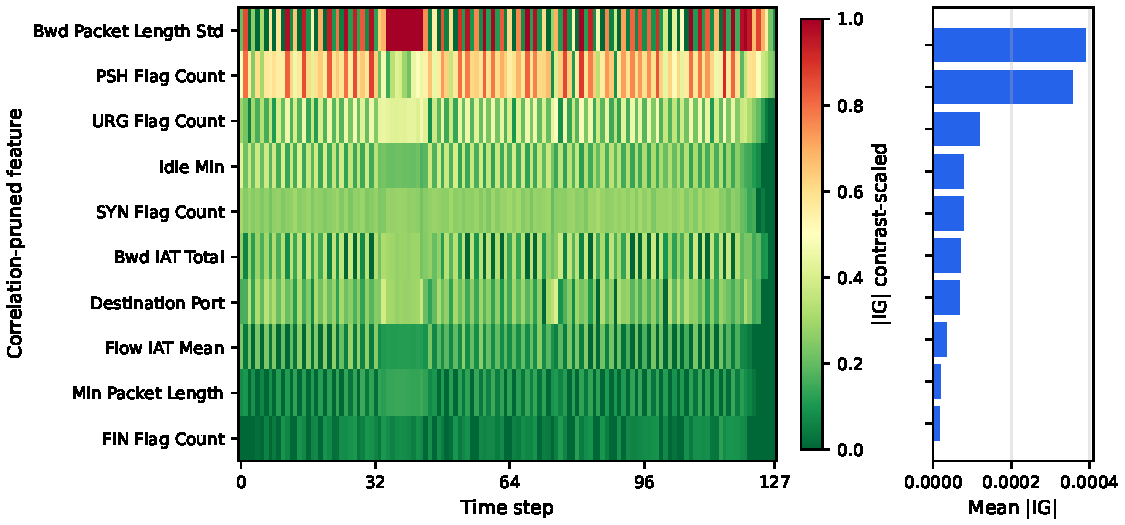
\includegraphics[width=0.96\textwidth]{figures/case_trace_attribution_heatmap_mainpaper.pdf}
  \Description{Case-level attribution heatmap for a detected DDoS window, with correlation-pruned non-redundant feature rows and time-step columns, plus a side bar of mean absolute integrated gradients.}
  \caption{Case-level attribution heatmap for a detected DDoS window. The case fused score is 0.506530, above the fixed threshold \(\tau=0.425420\); the benign-reference mean score is 0.3361. Rows show correlation-pruned non-redundant features ranked by mean absolute Integrated Gradients, and columns show time steps within the window. Correlation pruning is used only to reduce repetitive evidence display, not to establish statistical independence.}
  \label{fig:case_attribution_heatmap_main}
\end{figure*}

Masking provides a decision-level audit check. Figure~\ref{fig:case_masking_main} shows that masking top IG-ranked positions at $k=10$ and $k=20$ reduces the fused score below \(\tau\), flipping the decision to no alarm, while random masking remains above \(\tau\). This case provides an analyst-facing audit trace from score, to localized evidence, to masking-based decision change.

\begin{figure}[t]
  \centering
  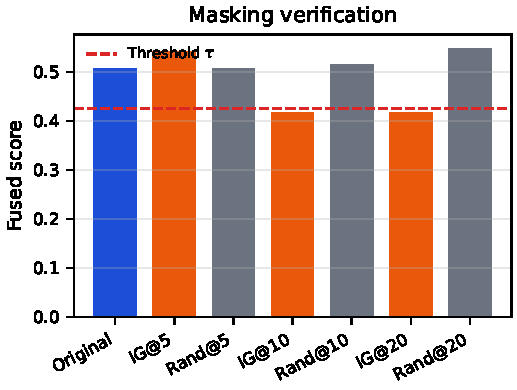
\includegraphics[width=\columnwidth]{figures/case_trace_masking_mainpaper.pdf}
  \Description{Masking-based decision verification for the selected DDoS case at fixed threshold tau; IG-guided masking at k=10 and k=20 falls below threshold while random masking stays above threshold.}
  \caption{Masking-based decision verification for the same DDoS case. The threshold \(\tau=0.425420\) is fixed. Masking top IG-ranked positions at \(k=10\) and \(k=20\) reduces the fused score below \(\tau\) and flips the decision to no alarm, while random masking remains above \(\tau\).}
  \label{fig:case_masking_main}
\end{figure}

\subsection{Fixed-Threshold Sensitivity Analysis}

Table~\ref{tab:noise_sensitivity} reports fixed-threshold sensitivity under Gaussian perturbation. Mild perturbation (\(\sigma=0.01\)) has limited effect on ranking performance, with AUC decreasing from 0.978349 to 0.977773 and AP decreasing from 0.963120 to 0.961328. However, fixed-threshold alarm metrics degrade under stronger perturbations. At \(\sigma=0.03\), Test FPR@\(\tau\) rises to 0.352003 and F1@\(\tau\) drops to 0.802693. At \(\sigma=0.05\), Test FPR@\(\tau\) rises to 0.963568 and F1@\(\tau\) drops to 0.603198.

The apparently counter-intuitive combination of high AUC/AP and high Test FPR@\(\tau\) is expected in this fixed-threshold sensitivity setting. AUC/AP summarize score ranking over possible thresholds, while Test FPR@\(\tau\) measures benign alarms at the clean-calibrated threshold. Under stronger perturbations, benign scores shift upward and many benign windows cross \(\tau\), causing high false positives. Attack scores can still remain ranked above benign scores on average, preserving AUC/AP. This indicates threshold miscalibration under perturbation rather than a contradiction between the metrics.

\begin{figure*}[t]
  \centering
  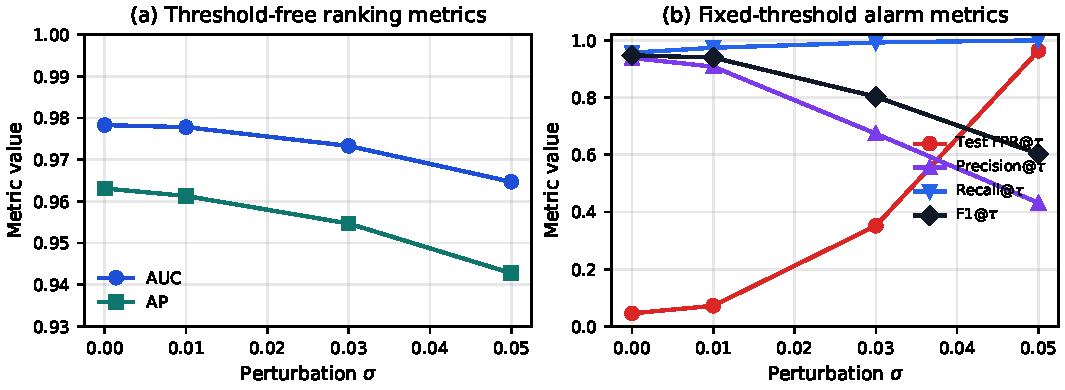
\includegraphics[width=0.96\textwidth]{figures/fixed_threshold_sensitivity_mainpaper.pdf}
  \Description{Two-panel trend plot under Gaussian perturbation: threshold-free ranking metrics AUC/AP and fixed-threshold metrics Test FPR at tau, precision at tau, recall at tau, and F1 at tau.}
  \caption{Fixed-threshold sensitivity under Gaussian input perturbation. The threshold \(\tau=0.425420\) is selected on the clean independent benign calibration split and then kept fixed for all perturbed test evaluations. AUC/AP decrease gradually, while Test FPR@\(\tau\) rises sharply and F1@\(\tau\) declines, indicating threshold miscalibration under perturbation.}
  \label{fig:fixed_threshold_sensitivity}
\end{figure*}

These results should be interpreted cautiously. The ranking quality is relatively stable under mild perturbation, but the calibrated threshold is not robust to larger distribution changes. Therefore, we do not claim strong robustness. In deployment, threshold calibration would need monitoring and possible recalibration when benign traffic changes.

\subsection{Supplementary Cross-Dataset Results}

Supplementary results on SWaT and UNSW-NB15 are reported as bounded transfer checks, not as co-equal evidence chains. Table~\ref{tab:cross_dataset_supplementary} summarizes the strict-protocol cross-dataset view with role annotations and the operating-point policy used for supplementary rows.

\begin{table*}[t]
  \centering
  \caption{Strict-protocol cross-dataset summary. CICIDS2017 is reported at the selected main operating point from the calibration sweep, while SWaT and UNSW-NB15 are reported at a fixed supplementary target\_fpr=0.05 to avoid dataset-specific favorable target selection; these rows are not intended as a direct cross-dataset ranking table.}
  \label{tab:cross_dataset_supplementary}
  \small
  \resizebox{\textwidth}{!}{%
  \begin{tabular}{llcccccccc}
    \toprule
    Dataset & Role & target\_fpr & AUC & AP & Test FPR & Precision & Recall & F1 & Interpretation \\
    \midrule
    CICIDS2017 & Primary calibrated evidence & 0.25 & 0.978349 & 0.963120 & 0.046023 & 0.938395 & 0.956847 & 0.947531 & Primary evidence \\
    SWaT & Supplementary ICS validation & 0.05 & 0.990444 & 0.997744 & 0.000000 & 1.000000 & 0.989982 & 0.994966 & Supplementary ICS check \\
    UNSW-NB15 & Distribution-shift stress test & 0.05 & 0.806125 & 0.754875 & 0.027463 & 0.240964 & 0.007032 & 0.013666 & Threshold-transfer failure \\
    \bottomrule
  \end{tabular}
  }
\end{table*}


SWaT is used as supplementary industrial-control validation. Table~\ref{tab:swat_supplementary_baselines} reports strict-protocol baseline comparison at target\_fpr=0.05; Ours reaches AUC 0.9904, AP 0.9977, Test FPR 0.0000, Precision 1.0000, Recall 0.9900, and F1 0.9950, providing supportive supplementary industrial-control evidence under the same calibration discipline. We interpret this as bounded evidence under one ICS setting, not as comprehensive validation across industrial-control environments.

\input{tables/table_swat_supplementary_baselines.tex}

UNSW-NB15 is treated as a distribution-shift stress test. Ours has non-trivial ranking (AUC 0.8061, AP 0.7549) but very low calibrated recall (0.0070) with F1 0.0137 at target\_fpr=0.05. This gap between ranking and thresholded recall indicates that a benign-calibrated threshold transferred from a different regime can fail even when score ordering remains partially informative. We therefore interpret UNSW-NB15 as explicit failure-mode evidence for threshold transfer, not as a success case.

The MLP row in the UNSW supplementary baseline table is a supervised window-label reference, whereas Ours and the anomaly baselines operate under benign-window anomaly-detection assumptions. Additional UNSW baseline details are kept as supplementary artifact material to preserve the main-text focus on the CICIDS2017 primary evidence chain.

For operating-point sensitivity outside CICIDS2017, we retain the strict two-point supplementary comparison (target\_fpr 0.05 and 0.15) as artifact-level evidence only; we do not present it as a full threshold sweep in the main text.

\subsection{Summary of Findings}

The CICIDS2017 strict-protocol results support three main findings. First, the proposed detector provides a strong calibrated operating point, achieving high recall and F1 while keeping observed benign FPR below 5\% on the test split. Second, the TAD score is most effective as a fused calibrated score, with feature deviation serving as the dominant signal and the critic adding complementary information. Third, the detector can provide auditable alarm evidence through time-step attribution, feature attribution, and masking-based decision checks.

At the same time, the results expose important limitations. Bot attacks are missed at the selected threshold. Fixed-threshold behavior is sensitive to stronger perturbations. Supplementary UNSW-NB15 results show very low recall under distribution shift, exposing a threshold-transfer limitation. These limitations motivate future work on attack-family-aware calibration, adaptive thresholding, and broader validation under realistic traffic shifts.

\section{Discussion and Limitations}\label{sec:discussion}

Table~\ref{tab:noise_sensitivity} evaluates fixed-threshold sensitivity under Gaussian perturbation. The ranking metrics degrade gradually under mild perturbation, while fixed-threshold decision quality becomes more sensitive under stronger perturbation; this supports a conservative deployment recommendation with drift monitoring and periodic recalibration.

\begin{table*}[t]
  \centering
  \caption{Fixed-threshold sensitivity under Gaussian input perturbation. The threshold \(\tau=0.425420\) is calibrated on the clean independent benign split and then kept fixed for all perturbed test evaluations.}
  \label{tab:noise_sensitivity}
  \small
  \resizebox{\textwidth}{!}{%
  \begin{tabular}{ccccccc}
    \toprule
    Perturbation \(\sigma\) & AUC & AP & Test FPR@\(\tau\) & Precision@\(\tau\) & Recall@\(\tau\) & F1@\(\tau\) \\
    \midrule
    0.0000 & 0.9783 & 0.9631 & 0.0460 & 0.9384 & 0.9568 & 0.9475 \\
    0.0100 & 0.9778 & 0.9613 & 0.0724 & 0.9078 & 0.9739 & 0.9397 \\
    0.0300 & 0.9733 & 0.9547 & 0.3520 & 0.6738 & 0.9925 & 0.8027 \\
    0.0500 & 0.9647 & 0.9428 & 0.9636 & 0.4319 & 0.9998 & 0.6032 \\
    \bottomrule
  \end{tabular}
  }
\end{table*}


The calibration implication is practical. A threshold that is well calibrated on one benign regime can drift under changed traffic conditions even when score ranking remains moderately stable. For deployment, this suggests a two-stage policy: monitor benign alarm rate continuously, and trigger recalibration when observed benign FPR exceeds an operational tolerance band for a sustained period.

Current evidence is intentionally compact and protocol-consistent. CICIDS2017 is the primary evidence chain, while SWaT and UNSW-NB15 are used to characterize operating boundaries under additional conditions rather than as co-equal primary benchmarks.

The study has four key limitations. First, Bot recall is zero at the selected CICIDS2017 operating point, showing attack-family coverage gaps despite strong aggregate metrics. Second, fixed-threshold behavior is sensitive under stronger perturbation, and UNSW-NB15 further exposes threshold-transfer failure under distribution shift. Third, the baseline suite is representative under strict protocol alignment, not exhaustive across all modern architectures. Fourth, audit evidence is lightweight and empirical: attribution-guided masking supports alarm-trace inspection, but does not prove complete faithfulness.

\subsection{Ethical Considerations and Open-Science Notes}
This work uses public benchmark traffic data and does not involve active attacks on operational systems. The main risk is overextending benchmark conclusions to production networks. We mitigate this risk by reporting observed benign FPR, explicit failure modes (including Bot miss and UNSW transfer failure), and strict calibration provenance.

The artifact structure is designed for reproducibility: strict split settings, calibration protocol, selected checkpoints, and table-generation scripts are recorded in the project outputs. We encourage deployment as analyst-assistive triage, not as a standalone replacement for security investigation workflows.

\section{Conclusion}

This paper presents a calibrated and auditable window-level NIDS pipeline based on TCN-WGAN-GP and fused TAD scoring under strict no-leakage evaluation. The primary evidence chain on CICIDS2017 shows that explicit independent benign calibration can deliver a strong operating point with low observed benign alarm rate while maintaining high recall and F1.

Beyond aggregate metrics, we provide attack-type and score-component analyses, plus lightweight auditability evidence through IG masking and a traceable single-window DDoS case. These analyses support a deployment-oriented claim: window-level anomaly scoring can be calibrated and inspected, not only ranked.

The paper also reports clear boundaries. Bot recall remains weak at the selected threshold, and fixed-threshold performance is sensitive under stronger perturbations. Supplementary SWaT and UNSW-NB15 results should be interpreted as bounded transfer evidence and stress-test limitations, not comprehensive cross-dataset generalization.

Future work should focus on attack-family-aware calibration, adaptive thresholding under drift, and broader multi-environment validation under the same strict protocol constraints.



\bibliographystyle{IEEEtran}
\bibliography{references}

\section*{LLM Usage Statement}
LLMs were used for editorial purposes in this manuscript, and all outputs were inspected by the authors to ensure accuracy and originality.

\end{document}
